\documentclass[10pt,a4paper,sans]{article}

\usepackage[utf8]{inputenc}
\usepackage{geometry}
\usepackage{helvet}
\usepackage[french]{babel}
\usepackage{graphicx}
\usepackage{xcolor}

\usepackage{titlesec}
\usepackage{enumitem}
\usepackage{pifont}

\usepackage[framemethod=tikz]{mdframed}
\usetikzlibrary{shadows}

\geometry{a4paper, top=0.75cm, left=0.75cm, right=1.0cm, bottom=1.0cm}

% Redéfinition format des titres/sections...
\titleformat{\section}[hang]
    {\Large\color{blue}\bfseries}
    {}
    {0em}
    {}[\titlerule]
\titlespacing{\section}{0cm}{0cm}{0.25cm}

\titleformat{\subsection}[hang]
        {\bfseries}
        {}
        {0em}
        {}[]
\titlespacing{\subsection}{0.25cm}{0.25cm}{0.25cm}

\titlespacing{\paragraph}{0.50cm}{0.12cm}{0.12cm}


%% Redéfinition format des listes
\setitemize[0]{label=\ding{226}, leftmargin=0.9cm, itemsep=0.05cm}

% Création des formats de cadres
\mdfdefinestyle{titre1}{backgroundcolor=lightgray}
\mdfdefinestyle{cadreCompetences}{backgroundcolor=lightgray, shadow=true, shadowcolor=black, 
          linewidth=1pt, linecolor=red, shadowsize=5.5pt, leftmargin=0pt, rightmargin=0pt, innerrightmargin=0pt}

\begin{document}

\hyphenrules{nohyphenation}

\begin{minipage}{0.36\textwidth}
    \input{contact}
\end{minipage}
\begin{minipage}{0.63\textwidth}
    \begin{mdframed}[style=titre1]
        \begin{flushright}
            \Large{\textbf{Ingénieur Mécanique}}
        \end{flushright}
    \end{mdframed}
    \begin{minipage}{0.75\textwidth}
        \subsection{Profil :}
        \begin{description}
            \item[Adaptable:]grande capacité d'apprentissage
            \item[Mobile:]possibilité de déplacement internationaux
            \item[Motivé]forte implication dans les projets
        \end{description}
    \end{minipage}
    \begin{minipage}{0.23\textwidth}
        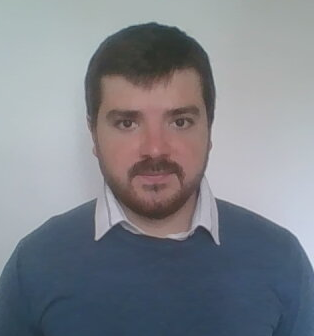
\includegraphics[width=\textwidth]{img/image_CV.png}
    \end{minipage}
\end{minipage}


\begin{minipage}[t]{0.25\textwidth}
    \begin{mdframed}[style=cadreCompetences]
        \section{LOGICIELS}
        \subsection{Dessin Technique}
        \begin{itemize}
            \item{Solidworks}
            \item{Unigraphics NX}
            \item{Autocad}
            \item{Creo/Pro E}
        \end{itemize}

        \subsection{Calcul numérique}
            \begin{itemize}
                \item{Solidworks}
                \item{NX + Nastran}
                \item{Octave/Matlab}
                \item{Scilab}
            \end{itemize}
        \subsection{Bureautique}
            \begin{itemize}
                \item{Excel}
                \item{Suite office}
                \item{latex}
            \end{itemize}

        \section{PROGRAM.}
        \subsection{Programmation application}
            \begin{itemize}
                \item{VBA
                    \hfill
                    
\includegraphics[scale=0.20]{img/star.png} \hspace{-0.2cm}
                    
\includegraphics[scale=0.20]{img/star.png} \hspace{-0.2cm}
                    
\includegraphics[scale=0.20]{img/star.png} \hspace{-0.2cm}
                    
\includegraphics[scale=0.20]{img/star.png} \hspace{-0.2cm}
                    
\includegraphics[scale=0.20]{img/star.png}}
                \item{Solidworks
                    \hfill
                    
\includegraphics[scale=0.20]{img/star.png} \hspace{-0.2cm}
                    
\includegraphics[scale=0.20]{img/star.png} \hspace{-0.2cm}
                    
\includegraphics[scale=0.20]{img/star.png} \hspace{-0.2cm}
                    
\includegraphics[scale=0.20]{img/half_star.png} \hspace{-0.2cm}
                    
\includegraphics[scale=0.20]{img/empty_star.png}}
                \item{Langage C}
            \end{itemize}
        \subsection{Développement Web}
            \begin{itemize}
                \item{HTML/CSS}
                \item{PHP}
            \end{itemize}

        \section{LANGUES}
        \subsection{Anglais: C1 (855-Toeic 2015)}
            \begin{itemize}
                \item{Compréhension}
                \item{Expression}
            \end{itemize}
        \subsection{Allemand : C1 (881-WIDAF 2015)}
            \begin{itemize}
                \item{Compréhension}
                \item{Expression}
            \end{itemize}

        \section{Loisirs}
            \begin{itemize}
                \item{squash, vélotourisme}
                \item{série tv, lecture}
                \item{robotique, développement web}
            \end{itemize}
    \end{mdframed}
\end{minipage}
\hfill
\begin{minipage}[t]{0.72\textwidth}
    \section{FORMATION}
        \begin{itemize}
            \item{2012--2016 : Diplome d'Ingénieur en Génie Mécanique INSA Strasbourg (Anciennement ENSAIS)}
            \item{2010--2012 : Classe Préparatoire intégrée INSA Strasbourg DeutschInsa (Moitié des enseignements en Allemand)}
            \item{Juin 2010 : Baccalauréat mention européenne Allemand Obtenu avec mention Bien}
        \end{itemize}

    \section{MILTON ROY : 1 entreprise, plusieurs expériences}
    \subsection{Juin 2018--Maintenant : Relais technique entre équipe agitation et Responsable Bureau d'Études}
    \begin{itemize}%
        \item Partage du temps de travail entre le site d’Avon (77) où travaille l’équipe Bureau d’Études agitation et Pont Saint Pierre (27)
        \item Maîtrise de Unigraphix NX et Autocad en autonomie
        \item Réalisation d’études d’agitation : Plans de détails, coupe, encombrement et gestion données ERP pour mise en production
        \item Voyage à Pune (Inde) en tant que consultant sur le dimensionnement mécanique pour le développement d’un outil automatique de chiffrage d’agitateurs.
        \item Formation de l’équipe Indienne pour le développement d’un marché local
    \end{itemize}

    \subsection{Juin 2017--Juin 2018 : Ingénieur Études Pompe doseusen}
    \begin{itemize}
        \item Maîtrise de Solidworks par un apprentissage en autonomie.
        \item Réalisation d’études pompe : Plans de détails, plans coupe, plans d’encombrements et gestion des données dans l’ERP pour mise en production
        \item Réalisation de calculs en soutien des projeteurs : échange thermique (analytique), fréquence propre(FEA), calcul contraintes (FEA et analytique), ...
        \item Projet d’automatisation des plans d’encombrement de pompe par macro Solidworks. Pilotage de Solidworks par Excel
    \end{itemize}

    \subsection{Septembre 2016--Juin 2017 : Participation au projet de tranfert de production de Samoreau(77) à Pont-Saint-Pierre(27)}
    \begin{itemize}
        \item Design des cuves et circuits hydrauliques des moyens d’essais pour agitateurs (verticaux et horizontaux).
        \item Développement d’outils d’analyse des données techniques de l’ERP pour tous les services (supply chain, documentation, production,...)
        \item Soutien technique pour l’adaptation des process et transfert des données techniques dans l’ERP (JD Edwards)
        \item Projet d’automatisation des nomenclatures (Excel) et plans d’encombrement d’agitateurs (format, SVG)
    \end{itemize}


    \subsection{2011--2016 : Stages dans différents sites de l'entreprise}
    \begin{itemize}
        \item Juin à Août 2011 – Samoreau (77) – Mesures des propriétés hydrauliques d’hélices d’agitateurs
        \item Mars à Août 2014 – Samoreau (77) – Améliorations de feuilles de calculs de dimensionnement d’agitateurs
        \item Juin à Août 2015 – Sunderland (Angleterre) – Design d’un nouvel espace de test pour compresseurs
        \item Mars à Août 2016 – Pont-Saint-Pierre (27) – Rationalisation d’une gamme de doseurs de pompes doseuses
    \end{itemize}
\end{minipage}

\end{document}
